
\chapter{Voorstudie}
\vspace{-3cm}
\section{Vereisten} \label{vereisten}
Alle bibliotheken en technologie\"{e}n die besproken zullen worden, moeten aan enkele voorwaarden voldoen. Zo moeten afbeeldingen en tekst verplaatst, geschaald, geroteerd en over elkaar geplaatst kunnen worden (wat dus inhoudt dat de gebruikte bibliotheek/technologie lagen moet ondersteunen). Idealiter kan tekst, eens op het canvas geplaatst, ook aangepast worden. Dit vooral om interactie met tekst voor de gebruikers gemakkelijker te maken. Nadien moeten de afbeeldingen ge\"{e}xporteerd en hun properties (tekst, KPI's etc.) bewaard kunnen worden. Aangezien KPI's aanwezig zijn op de afbeelding, moeten deze later nog aangepast kunnen worden. De afbeeldingen zullen dus om de zoveel tijd opnieuw gerenderd worden met aangepaste KPI`s. Dimensies van omslagfoto's kunnen redelijk groot uitvallen. Twitter verwacht bijvoorbeeld een afbeelding van 1500 op 500 pixels. Dit is natuurlijk niet gebruiksvriendelijk weer te geven in een browservenster. Daarom moet herschalen van het volledige canvas met elk van zijn objecten mogelijk zijn. Hierbij is het belangrijk dat alle verhoudingen behouden blijven om uiteindelijk dezelfde afbeelding te bekomen zoals die door de gebruiker gemaakt werd. Naast de frontend manipulatie van afbeeldingen zal ook manipulatie in de backend onderzocht moeten worden.  

\section{Frontend afbeelding manipulatie}
\subsection{Fabric.js}
Redelijk wat bilbiotheken om afbeeldingen te manipuleren zijn beschikbaar. De meeste hiervan zijn gericht op het gebruiken van filters op afbeeldingen of het maken van animaties in een canvas. Hoewel deze bibliotheken veel te bieden hebben, zijn ze minder geschikt voor deze toepassing. Het is hier namelijk de bedoeling om elementen op een canvas te positioneren, zowel tekst als afbeeldingen en deze op gepaste wijze op te slaan. 

Een bibliotheek die onmiddellijk veelbelovend lijkt te zijn is Fabric.js. Het is een JavaScript bibliotheek die HTML5 canvas manipulatie gemakkelijker maakt. Het maakt het mogelijk om object-geori\"{e}nteerd te werken binnen een canvas in plaats van simpelweg te `tekenen' op het canvas. Dit maakt het veel gemakkelijker om met deze objecten te werken. Selecteren, verplaatsen, herschalen, roteren en dergelijke transformaties kunnen ondernomen worden zonder veel problemen. 

\textbf{Functionaliteit} \break 
In plaats van te functioneren op de context van het canvas zal Fabric gebruik maken van objecten die aan het canvas toegevoegd worden \cite{FabricJSDocs}. Fabric bezit zeven verschillende standaard vormen: 

\begin{itemize}
	\item Cirkel
	\item Ellips
	\item Lijn
	\item Polygon
	\item Polylijn
	\item Rechthoek
	\item Driehoek
\end{itemize}

Alle objecten erven over van het \textit{root object}. Dit stelt een tweedimensionale vorm voor in het tweedimensionaal canvas en bezit een positie in het canvas (x-en y-co\"{o}rdinaat), een hoogte en een breedte. Aangezien elk objct dus overerft van deze klasse, ontstaat een soort van hi\"{e}rarchie en kunnen methodes geschreven worden die bruikbaar zijn voor elke instantie van een object \cite{FabricJSIntro}. 

Interessanter voor deze implementatie zijn de tekst en afbeelding objecten. Naast het gewone fabric.Text object, wat enkel statische tekst voorstelt, is ook de fabric.IText beschikbaar. Met dit object kan interactieve tekst aan het canvas toegevoegd worden. Deze tekst kan dus in het canvas zelf aangepast worden. Het Text object bezit properties om grootte, stijl (vet/schuin/normaal), gewicht en de familie (font type) aan te passen. Het standaard HTML canvas bezit slechts twee methodes om tekst te renderen: \lstinline|{strokeText(text, x, y [, maxWidth])}| en \lstinline|{fillText(text, x, y [, maxWidth])}| \cite{MozillaCanvas-DrawingText}. De eerste methode zal ingevulde tekst op het canvas tekenen op de meegegeven x-en y-positie. De tweede zal enkel de omtrek van de meegegeven tekst op het canvas tekenen. Naast deze methodes zijn ook enkele properties beschikbaar zoals font (e.g. 20px comic-sans), textAlign (e.g. center), textBaseline (e.g. alphabetic) en direction (e.g. ltr). Functionaliteit hiervan is eerder beperkt. Zeker niet uitgebreid genoeg om aan de gestelde eisen (zie sectie \ref{vereisten}) te kunnen voldoen. 

Het tekst object die Fabric voorziet voegt heel wat nieuwe functionaliteit toe zoals: 

\begin{itemize}
	\item Multiline ondersteuning
	\item Tekst achtergrond
	\item Tekst decoratie
	\item Uitlijning
	\item Lijnhoogte
\end{itemize}

Vooral ondersteuning van multiline tekst en uitlijning hiervan zijn zeer handige \textit{features}. Alle objecten op het canvas kunnen \textit{by default} geselecteerd en verplaatst worden. Natuurlijk is dit met het standaard canvas element ook mogelijk, maar code hiervoor zou steeds complexer worden naarmate meer functionaliteit toegevoegd wordt. Daarom is onderzoek naar een gepaste bibliotheek hier zeker niet misplaatst. Wordt even stilgestaan bij het \textit{draggable} of verplaatsbaar maken van tekst in een standaard HTML canvas, is al snel duidelijk dat hier heel wat code voor nodig is. 

Alle tekst, die op het canvas geplaatst wordt, moet bijgehouden worden in een lijst of array. Wanneer een \textit{mouse-down} event plaatsvindt, moet berekend worden of de klik daadwerkelijk op een item in het canvas gebeurde. Is dit het geval dan moet de index van het geselecteerde item opgeslagen worden. Bij het triggeren van een \textit{mouse-move} event moeten de co\"{o}rdinaten van dit item aangepast worden naar deze van de cursor, waarna ieder item terug op het canvas getekend moet worden. 

\begin{lstlisting}[language=javascript]
	document.getElementById('addTextButton').click(function() {
	 var text = document.getElementById('text').value;
	 items.push(text);
	});
	
	document.getElementById('canvas') on mouse down (
	 // Kijk wanneer positie van de cursor overeen komt met een tekst object
	)
\end{lstlisting}

Ook afbeeldingen zijn gemakkelijk te manipuleren in een Fabric canvas. Afbeeldingen kunnen geladen worden vanuit een Scalable Vector Graphics (SVG) element, een object of een URL. Met het standaard canvas element kunnen enkel afbeeldingen via URL ingeladen worden. Hoewel dit bij deze toepassing op zich niet onmiddellijk een bottleneck vormt aangezien de afbeelding ingeladen zal worden vanuit een `file server', kan het toch handig zijn om de extra functionaliteit ter beschikking te hebben. In de toekomst kan het bijvoorbeeld nodig zijn om een SVG afbeelding te cre\"{e}ren en in te laden in het canvas. Dan moet, bij het gebruik van Fabric, geen ander script/bibliotheek ge\"{i}nstalleerd worden om deze functionaliteit te verkrijgen. Het fabric.Image object bezit heel wat methodes die het gebruik van afbeeldingen net dat beetje eenvoudiger maken. De \lstinline{scaleToWidth()} functie kan gebruikt worden om de afbeelding de volledige breedte van het canvas te laten innemen. Manipulatie van een object kan ook afgesloten worden. 
%Zo zijn er de \lstinline{lockMovementX()}, \lstinline{lockMovementY()}, \lstinline{lockScalingX}, \lstinline{lockScalingY} en \lstinline{lockRotation} methodes die bij het renderen van achtergrondafbeeldingen zeer nuttig kunnen zijn. Het is namelijk handig om de acties van de gebruiker wat in te kunnen perken. Door enkele bewegingen te locken wordt het dus onmogelijk om bijvoorbeeld de afbeelding uit het zichtbare gedeelte van het canvas te slepen. 
Naast de mogelijkheid tot inladen van afbeeldingen, kunnen hierop ook filters toegepast worden. Hoewel dit momenteel geen vereiste is voor het project, zou dit in de toekomst toegevoegd kunnen worden. Enkele filters die beschikbaar zijn voor een Image object zijn:  

\begin{itemize}
	\item Helderheid
	\item Contrast
	\item Grijstinten
	\item Omkeren
	\item \textit{Pixelate}
	\item Sepia
	\item Ruis
\end{itemize}

Een belangrijke vereiste is de ondersteuning van lagen aangezien tekst bovenop de afbeelding geplaatst moet kunnen worden. Hiervoor bezit Fabric verschillende methodes. Objecten kunnen een positie hoger of lager in de stack van objecten, die op dat moment op het canvas aanwezig zijn, geplaatst worden met behulp van de \lstinline|sendBackwards(object)| of \lstinline|bringForward(object)| methodes. Deze methodes bezitten een optionele \textit{intersecting} parameter \lstinline{(boolean)} die het object net voor of na het volgende snijdende object in de stack zal plaatsen. 

%AFBEELDING!!!!

Het canvas bezit ook twee methodes om objecten volledig onderaan of bovenaan de stack te plaatsen: \lstinline{sendToBack(object)} en \lstinline{bringToFront(object)}. Deze methodes zijn perfect om de afbeelding in te stellen als achtergrond van het canvas. Naast deze methodes bezit het canvas ook een belangrijke property, \lstinline{preserveObjectStacking}. Wanneer \lstinline{true} zal de positie van alle objecten op de stack bewaard blijven. Dit zorgt er voor dat objecten niet plots bovenaan de stack komen te staan als ze geselecteerd worden. Voor uitwerking van het project is de mogelijkheid tot het gebruiken van lagen onontbeerlijk. Het standaard canvas element bezit deze functionaliteit niet, althans niet zo naadloos ge\"{i}mplementeerd. 
%Het is wel mogelijk met wat tricks (zie sectie over vanilla js/jquery).

Misschien een van de grootste voordelen van Fabric is dat het zelf zorgt voor het renderen van het canvas wanneer een object gemanipuleerd wordt en dat de state van het canvas bijgehouden wordt. Kortweg betekend dit dat de \lstinline{canvas.draw()} functie niet telkens moet aangeroepen worden wanneer een manipulatie plaatsvindt. 

\textbf{Gebruiksgemak} \break
Fabric blijkt een erg veelzijdige bibliotheek te zijn die over zeer veel features beschikt die allen kunnen bijdragen tot een gebruiksvriendelijke implementatie. Gebruik van deze bibliotheek is eenvoudig (straightforward) en intu\"{i}tief. Na het aanmaken van een canvas object, kan een toegevoegd object onmiddellijk verplaatst, geschaald en geroteerd worden. Dit is een grote hulp tijdens het ontwikkelen, vergeleken met het standaard canvas element waarvoor meerdere event listeners aangemaakt moeten worden om gelijkaardige functionaliteit te verkrijgen. 

Belangrijk bij het gebruik van bibliotheken zijn de ondersteunde browsers \cite{Fabricsupportedbrowsers}. Fabric wordt ondersteund door volgende browsers: 
\begin{itemize}
	\item Firefox 2+
	\item Safari 3+ 
	\item Opera 9.64+
	\item Chrome (alle versies)
	\item IE10, IE11 en Edge
\end{itemize}

De Fabric bibliotheek ondersteund ook \textit{touch events} waardoor gebruik op mobiele apparaten geen probleem is. 

\textbf{Serialisatie} \cite{FabricJSIntro3Serialization} \break 
Geannoteerde afbeeldingen moeten ook opgeslagen kunnen worden. Een Fabric canvas kan op verschillende manieren ge\"{e}xporteerd worden. Fabric bezit twee basismethodes voor de serialisatie van een canvas: \lstinline{toObject()} en \lstinline{toJSON()}. De \lstinline{toJSON()} functie geeft een JavaScript Object Notation (JSON) object terug die er als volgt uitziet:

\begin{lstlisting}[language=javascript]
 {"objects": [], "background": "rgba(0,0,0,0)"}
\end{lstlisting} 

De \textit{objects} eigenschap bevat alle informatie over de objecten die aanwezig zijn op het canvas zoals tekst, afbeeldingen en vormen. \textit{background} geeft de kleur van het canvas weer. 

%// Mss vergelijking maken tussen output van json vs output van png (canvas.toDataUrl(‘png’))

De \lstinline{toObject()} methode geeft hetzelfde terug als \lstinline{toJSON()} maar dan als een object. Het verkregen object is eigenlijk het resultaat van het aanspreken van de \lstinline{toObject()} methode van elk element op het canvas. Bij het omzetten van een element naar een object, kan meegegeven worden welke eigenschappen het object moet bevatten via de optionele \lstinline{propertiesToInclude} parameter. Wanneer een nieuwe klasse wordt toegevoegd, kan dus simpelweg de \lstinline{toObject()} methode aangepast of uitgebreid worden. In de scope van dit project kan deze functionaliteit gebruikt worden om een extra eigenschap aan een object te geven die aangeeft of een object een KPI voorstelt of gewoon tekst.  

\begin{lstlisting}[language=javascript]
	text.toObject = (function(toObject) {   
	return function() {     
		return fabric.util.object.extend(toObject.call(this), {       
				kpiType: this.kpiType     
			});   
		}; 
	})(text.toObject);
\end{lstlisting}

Naast het omzetten van een canvas naar JSON of een object, kan een canvas ook als SVG ge\"{e}xporteerd worden met behulp van de \lstinline{toSVG()} methode. Deze methode kan net zoals de \lstinline{toObject()} methode uitgebreid worden. Het voordeel van het exporteren als SVG-bestand is dat het zonder aanpassing gebruikt kan worden in een browser of applicatie die SVG ondersteunt. Zowel JSON als het object moeten eerst in een canvas geladen worden om ze weer te geven. 

Natuurlijk is het ook mogelijk om een canvas als afbeelding te exporteren. Via de \lstinline{toDataUrl()} methode kan het canvas zowel als JPEG als PNG opgeslagen worden. Als parameter aan deze functie kunnen volgende opties meegegeven worden:

\begin{itemize}
	\item format (PNG of JPEG)
	\item quality (waarde tussen 0 en 1, enkel voor JPEG)
	\item multiplier (waarde waarmee de afbeelding geschaald moet worden)
	\item left (linker offset om bij te snijden/crop)
	\item top (offset bovenaan om bij te snijden)
	\item width 
	\item height
\end{itemize}

Omdat afbeeldingen ook KPI's kunnen bevatten, kunnen ze niet onmiddellijk ge\"{e}xporteerd worden als afbeelding. Ook moet rekening gehouden worden met de grootte van de bestanden wanneer deze terug naar de server gezonden worden. In een tekst bestand kan nu eenmaal veel meer informatie gestoken worden dan in een afbeelding van dezelfde grootte. 

Vanuit een JSON string of een SVG element kan een canvas opnieuw opgesteld worden \cite{SVGElement}. Voor beide representaties zijn twee methodes beschikbaar. JSON kan terug ingeladen worden met behulp van de \lstinline{loadFromJSON()} of \lstinline{loadFromDatalessJSON()} methodes, die beiden op het canvas zelf aangeroepen worden. \lstinline{loadFromJson()} zal zoals verwacht gewoonweg een JSON string in het canvas laden. \lstinline{loadFromDatalessJSON()} kan gebruikt worden bij het inladen van complexe Path objecten. Een pad zal heel wat informatie bevatten, die een JSON string al snel onleesbaar en gigantisch lang kan maken. Bij het inladen van een dataless JSON string zullen de complexe Path objecten via een SVG bestand opgehaald worden. Door het reduceren van lange paden tot een eenvoudig pad naar het SVG bestand is de representatie van het canvas veel compacter geworden. SVG elementen worden ingeladen via de \lstinline{loadSVGFromURL()} methode, die als parameter een link naar de SVG inhoud verwacht. 


\subsection{Konva.js} 
Konva is een HTML5 Canvas JavaScript \textit{framework} dat voor zowel desktop als mobiele applicaties extra functionaliteit aan het canvas toevoegt. Vormen kunnen aan een canvas toegevoegd worden waarna deze verplaatst, herschaald en geroteerd kunnen worden. Konva startte als een GitHub fork van KineticJS, een andere HTML5 Canvas bibliotheek. Helaas wordt KineticJS momenteel niet meer onderhouden, alhoewel de laatste release wel nog gedownload kan worden. Stabiele releases zijn nog steeds beschikbaar alsook een lichtere versie van KineticJS, genaamd Concrete.js. Het bespreken van KineticJS op zich wordt hier achterwege gelaten aangezien het niet langer onderhouden wordt en vooral gericht is op het tekenen en animeren in een canvas.
%(en Konva hier toch op gebaseerd is) 

\textbf{Functionaliteit} \break
Konva bezit van een element, de stage, die gebruikt wordt als basis van een project. Deze stage kan meerdere lagen bevatten, die op hun beurt andere objecten of groepen van objecten bevatten. Elke laag in de stage bezit twee canvas \textit{renderers}. Een \textit{renderer} zal instaan voor het weergeven van alle objecten, dit is dus een canvas die instaat voor de visualisatie. De andere is een zogenaamde \textit{hit graph renderer}, dit is in principe een verborgen canvas dat instaat voor event detectie. Wanneer een bestaand object op het canvas wordt aangeklikt zal dus een event getriggerd worden op het verborgen canvas waarna deze opgevangen kan worden. Naast standaard objecten zoals rechthoeken, tekst, polygonen en afbeeldingen bezit Konva ook de Shape klasse waarmee aangepaste vormen aangemaakt kunnen worden. Elk van deze objecten zijn uitbreidingen op het Konva.Node object. In de context van Konva is een node een object dat in een laag geplaatst en aangepast kan worden. 

Objecten kunnen versleepbaar gemaakt worden door de \textit{draggable} attribuut op \lstinline{true} te zetten. Zoals verwacht kunnen afbeeldingen, lijnen, objecten en groepen van objecten versleept worden op een laag maar ook de stage bezit de \textit{draggable} eigenschap. De volledige stage, inclusief alle lagen en hun objecten kunnen zo versleept worden. In principe is dit een soort pan over het canvas. Aan een object kunnen ook enkele \textit{event handlers} gebonden worden die drag \& drop events detecteren. Beschikbaar zijn een \lstinline{dragstart}, \lstinline{dragmove} en \lstinline{dragend} event. 

Tekst kan op twee manieren weergegeven worden op een laag. Met het Konva.Text object kan een string aangemaakt worden met allerlei verschillende eigenschappen. Enkele van deze eigenschappen zijn: 

\begin{itemize}
	\item fontFamily
	\item fontSize
	\item fontStyle
	\item fontVariant (normal of small-caps)
	\item align (links, rechts of gecentreerd)
	\item lineHight 
	\item wrap (woord, karakter of niets)
	\item fill
	\item stroke
\end{itemize}

Het Konva.TextPath object bezit grotendeels dezelfde eigenschappen als het gewone Text object maar plaatst de tekst op een meegegeven pad. Dit pad wordt meegegeven als een eigenschap in de vorm van een SVG string. Op deze manier kan tekst bijvoorbeeld op de rand van een cirkel geplaatst worden. 

Afbeeldingen kunnen op de stage getoond worden via het Konva.Image object. Deze verwacht een HTML5 Image element als parameter. Optioneel kunnen een x-en y-positie, hoogte, breedte, id, naam en een object om de afbeelding bij te snijden, meegegeven worden. Ook vanuit een URL kan een afbeelding in een Konva.Image object geladen worden. Filters zoals \textit{blur}, helderheid, RGBA, HSV/HSL, \textit{emboss}, \textit{enhance}, \textit{gradient}, inverteren, grijstinten en patronen kunnen allen op een afbeelding toegepast worden. Verder kunnen afbeeldingen, net zoals alle andere objecten versleepbaar gemaakt worden in de laag waar ze getekend zijn. 

Zoals eerder vermeld maakt Konva gebruik van lagen waarin objecten geplaatst kunnen worden. Dit zorgt er niet enkel voor dat objecten over elkaar getekend kunnen worden maar het is een zeer goede manier om het tekenen van objecten performant te houden. Lagen zullen pas opnieuw getekend/gerendered worden wanneer een object in die laag aangepast wordt. Zo kan een laag enkel statische elementen bevatten, terwijl een andere laag dynamische elementen bevat. Het is namelijk zinloos en helemaal niet performant om elke laag, dus ook deze waar niets in veranderde, opnieuw te tekenen wanneer een element ge\"{u}pdatet wordt. Het werken met lagen wordt in Konva mogelijk gemaakt door voor elke laag een nieuw canvas element in het Document Object Model (DOM) aan te maken. Binnen een laag kunnen objecten elkaar ook overlappen. 

\'{E}\'{e}n van de vereisten voor het project was de mogelijkheid tot (intu\"{i}tief) herschalen van objecten op het canvas. Aan een afbeelding kunnen in elk van de hoekpunten ankers toegevoegd worden. Deze dienen als referentiepunten om de eigenschappen van de afbeelding te manipuleren. Deze ankers krijgen events toegewezen die, eens getriggerd, het object tijdelijk niet langer versleepbaar maken en de transformatie zullen afhandelen. X-en y-posities zullen ge\"{u}pdatet worden waarna de laag opnieuw getekend wordt. Mits wat programmeerwerk is het herschalen van afbeeldingen in het canvas dus haalbaar. Een ander verhaal is het transformeren van tekst. Dit kan enkel via de fontSize eigenschap van het Konva.Text object. Natuurlijk zou het mogelijk zijn hier ook ankers aan te koppelen die dan invloed hebben op de grootte van de tekst. Dit zal logischerwijze niet gunstig zijn voor de performantie van de applicatie (extra event \textit{listeners}, berekenen van nieuwe posities en bijhorende tekst grootte, opnieuw tekenen van tekst met nieuwe eigenschappen etc.). %//HIT-TESTING buzzword

%\subsubsection*{Caching}
Om performantie van het canvas te verbeteren, bezit Konva caching. Iedere node kan gecached worden om vlugger veranderingen aan het canvas af te kunnen handelen. Gecachete nodes worden omgezet in afbeeldingen die in een buffer canvas opgeslagen worden. Bij transformaties in het canvas kunnen deze buffer afbeeldingen gebruikt worden. Vooral bij complexe elementen zoals tekst of vormen met schaduwen kan caching een groot verschil maken. 

Wat Konva mist qua functionaliteit is interactieve tekst. Hiermee wordt tekst bedoeld die rechtstreeks in het canvas aangepast kan worden. Dit heeft vooral invloed voor het gebruiksgemak van de applicatie. Het is namelijk intu\"{i}tiever om tekst in het canvas aan te passen door het te selecteren dan het via een input kader te doen. Gebruikers zullen sneller de tekst zelf proberen selecteren om deze aan te passen dan het object te selecteren en in een input veld de aanpassingen te maken om uiteindelijk nog de veranderingen door te moeten voeren door middel van een submit knop. 

\newpage
\textbf{Gebruiksgemak} \break
Konva is een veelzijdige bibliotheek die manipulatie van het tweedimensionale HTML canvas mogelijk maakt met JavaScript. In de standaard bibliotheek is genoeg functionaliteit beschikbaar om complexe canvas interacties mogelijk te maken. Naast verschillende standaard objecten zoals rechthoeken, cirkels, lijnen, afbeeldingen en tekst kunnen nieuwe vormen eenvoudig aangemaakt worden (en dit zowel op desktop als op mobiel.)
%// Konva maakt het tekenen van complexe grafische elementen op <canvas> mogelijk
% INSERT VOORBEELDCODE!!

\textbf{Serialisatie} \break
Om de stage op te kunnen slaan, kan deze ge\"{e}xporteerd worden als JSON met behulp van de \lstinline{toJSON()} functie. Een JSON object ziet er als volgt uit:

\begin{lstlisting}[language=javascript]
	{
	  "attrs": {
	    "width": 578,
	    "height": 200
	  },
	  "className": "Stage",
	  "children": [
	    {
	      "attrs": {},
	      "className": "Layer",
	      "children": [
	        {
	          "attrs": {
	            "width": "auto",
	            "height": "auto",
	            "text": "Hello World!",
	            "fontFamily": "Arial",
	            "fontSize": 70,
	            "x": 100,
	            "y": 100,
	            "stroke": "white",
	            "strokeWidth": 2,},
	          "className": "Text"
	        },
	        {
	          "attrs": {
	            "x": 100,
	            "y": 100,
	            "width": 200,
	            "height": 10,
	            "fill": "black",
	            "rotation": 0.7,
	            "id": "rectangle"
	          },
	          "className": "Rect"
	        }]
	    }
	  ]
	}
\end{lstlisting}

Elk object bezit dus attributen (attrs), de naam van de klasse (className) en zijn child objecten (children).  De attributen bevatten de eigenschappen van het object zoals hoogte, breedte, id, x-en y-co\"{o}rdinaten, stijlinformatie en rotatiehoek. Alle objecten die naar dit ene object refereren en dus zijn children zijn, zitten in het children attribuut. Wordt bijvoorbeeld gekeken naar de stage, het eigenlijke canvas die de andere objecten bevat, dan is het duidelijk dat alle andere objecten tot de children van dit object behoren. In bovenstaand voorbeeld bevat de stage \'{e}\'{e}n laag die op zijn beurt een tekst object en een rechthoek bevat \cite{KonvaSerialize}. %(Niet enkel de stage maar ook alle nodes kunnen zelf als JSON geëxporteerd worden. )

Om vanuit een JSON object een stage te cre\"{e}neren, moet eerst en vooral een nieuwe node aangemaakt worden. Met behulp van de \lstinline{Konva.Node.create()} methode kan vanuit het JSON object een stage aangemaakt worden. 
\begin{lstlisting}[language=HTML]
	<div id="container"></div>
	<script>
		var stage = Konva.Node.create("JSON", "container");
	</script>
\end{lstlisting}

Bevat een stage afbeeldingen of events, dan moeten deze opnieuw aangemaakt worden en met behulp van de \lstinline{get()} methode en selectors ingesteld worden. Dit kan als volgt uitgevoerd worden \cite{KonvaLoad}:

\begin{lstlisting}[language=javascript]
	var image = new Image();
    image.onload = function() {
        stage.get('#image')[0].image(image);
        stage.draw();
    };
    image.src = '/image.jpg';
\end{lstlisting}

Om een stage te exporteren als afbeelding kan gebruik gemaakt worden van de \lstinline{toDataURL()} methode. Dit zal een URL teruggeven die voorafgegaan wordt door de data van de afbeelding. Standaard is dit een PNG afbeelding die base64 gecodeerd wordt. Via parameters kunnen het type van de afbeelding (JPEG/PNG), x-en y-co\"{o}rdinaten, hoogte, breedte en kwaliteit (enkel van toepassing bij JPEG) ingesteld worden. Belangrijk hierbij is dat afbeeldingen zich op een webserver moeten bevinden op hetzelfde domein als waar de uitgevoerde code staat \cite{KonvaToImage}. 

\subsection{EaselJS}
EaselJS is \'{e}\'{e}n van de bibliotheken behorende tot de CreateJS suite. CreateJS is een verzameling van \textit{open source} bibliotheken en tools om interactieve web applicaties te maken. Zo bezit CreateJS ondermeer bibliotheken voor het cre\"{e}ren van animaties (TweenJS), om te werken met audio (SoundJS) en om het laden van data in een applicatie te regelen (PreloadJS). EaselJS maakt interactie met het HTML5 canvas element in JavaScript zeer eenvoudig. Het is een zeer krachtige bibliotheek die ondersteuning biedt voor zowel statische afbeeldingen als animaties. Ook bezit het enkele experimentele features om onder andere HTML elementen te beheren alsof ze deel uit maken van het canvas zelf. Dit kan handig zijn om een elementen bovenop het canvas te plaatsen, zonder dat deze tot het canvas zelf behoren, zoals een toolbar die een tekst editor bevat. 

\textbf{Functionaliteit} \break
De basis van de Easel workflow is het Stage object. Dit object wordt opgebouwd op basis van een HTML canvas element en zal alle objecten bevatten die op het canvas getoond moeten worden. De stage bevat een \lstinline{tick()} methode die, wanneer opgeroepen, alle objecten op het canvas zal renderen. Een Ticker klasse zorgt voor een gecentraliseerde tick, waarop \textit{listeners} kunnen subscriben. In de \textit{listeners} worden objecten in de stage verandert en wordt de stage ge\"{u}pdatet via de \lstinline{update()} methode. Omdat Easel zelf geen specifieke functionaliteit bezit om objecten te kunnen verslepen, moet dit gebeuren aan de hand van events. Zo zijn er de \lstinline{mousedown}, \lstinline{mouseup}, \lstinline{pressmove} en \lstinline{pressup} events die het mogelijk maken om objecten te verslepen over het canvas. Na het aanmaken van een event \textit{listeners} op het \lstinline{pressmove} event, kan een stuk code geschreven worden die de positie van het object aanpast naar de huidige positie van de cursor. Door telkens het canvas up te daten (met de \lstinline{update()} methode) wanneer de positie verandert, kan de \textit{drag \& drop} functionaliteit bekomen worden \cite{EaselMouseInteraction}.  

Met de Text klasse kan tekst op het canvas geplaatst worden. Aan de constructor kunnen verschillende parameters meegegeven worden waaronder tekstkleur, lettertype, lijnhoogte, lijnbreedte, omlijning, rotatie en type uitlijning. Daarnaast kunnen ook de positie, schaal, zichtbaarheid en dergelijke meegegeven worden. Met behulp van eerder besproken event \textit{listeners}, kunnen tekst objecten versleepbaar gemaakt worden. Wat deze klasse niet bezit is mogelijkheid tot het aanpassen van tekst in het canvas. In principe kan dit ge\"{i}mplementeerd worden met behulp van de DOMElement klasse. Dit is de experimentele klasse waarmee HTML elementen aangepast kunnen worden alsof ze zich in het canvas zelf bevinden. Een tekst input kan dan over het canvas geplaatst worden en met behulp van extra event \textit{listeners} en styling (om het input veld onzichtbaar te maken), kan deze input aan een Text object gebonden worden. 

Afbeeldingen kunnen worden weergegeven op het canvas met de Bitmap klasse. Deze klasse kan naast afbeeldingen ook een canvas of een video weergeven. Als parameter kan een HTML \textit{image}, canvas of video element meegegeven worden of simpelweg de Uniform Resource Identifier (URI) naar de afbeelding \cite{URI}. Wanneer een afbeelding/video/canvas geladen wordt via de URI, dan zal een nieuw Image object aangemaakt worden en zal dit meegegeven worden aan de \textit{image} eigenschap van het Bitmap Object. Via de \lstinline{setTransform()} methode kunnen x-en y-positie, schaal, rotatie en helling van het object aangepast worden \cite{EaselDocs}. 

Easel ondersteunt het direct schalen van objecten in het canvas niet. Om dit toch te verwezenlijken, moet een input gedefinieerd worden die de schaal van het object in kwestie zal aanpassen. Deze schaal kan aangepast worden met behulp van de \lstinline{scaleX} en \lstinline{scaleY} eigenschappen van het object. Na iedere verandering zal de stage ge\"{u}pdatet moeten worden. Natuurlijk is dit ook mogelijk door gebruik te maken van de JQuery \lstinline{resizable()} methode. Hier moet dan opnieuw gebruik gemaakt worden van de experimentele DOMElement klasse om een element te beheren dat zich buiten het Easel canvas bevindt. 

\textbf{Gebruiksgemak} \break
Complexe objecten zoals afbeeldingen en tekst vergen veel om te renderen. Daarom is het best om deze objecten te cachen. Wanneer de \lstinline{cache()} methode aangeroepen wordt op een object wordt het object in een nieuw canvas geplaatst. Dit nieuwe canvas zal dan telkens gebruikt worden wanneer een aanpassing in het originele canvas gebeurt. Het spreekt voor zich dat gecachete objecten enkel gebruikt kunnen worden bij basistransformaties zoals verplaatsingen en rotaties. Bij complexere transformaties zoals herschalen of het toepassen van filters dient de cache opnieuw ge\"{u}pdatet te worden. Aan de \lstinline{cache()} methode kunnen x-en y-co\"{o}rdinaten, hoogte, breedte en schaal meegegeven worden. Deze parameters defini\"{e}ren het gebied dat gerendered en gecachet zal worden. 
%https://jsfiddle.net/xnqcjsg8/1/

EaselJS wordt ondersteund door elke browser die het HTML Canvas element ondersteunen. De meest recente browsers ondersteunen het canvas element en zijn dus perfect compatibel met EaselJS. In Internet Explorer 11 kan het canvas niet ge\"{e}xporteerd worden met de \lstinline{toDataURL()} methode wanneer afbeeldingen aanwezig zijn op het canvas. Aangezien het canvas niet opgeslagen dient te worden als afbeelding maar als JSON vormt dit niet onmiddellijk een probleem.

\newpage
\textbf{Serialisatie} \break
Easel bezit geen functionaliteit om een stage te exporteren. Voor dit project in het bijzonder is dit natuurlijk een zeer groot nadeel. Als een stage niet ge\"{e}xporteerd of geserialiseerd kan worden, kan deze niet opgeslagen worden. Natuurlijk is het nog steeds mogelijk om een stage te exporteren. Alle \textit{children} van de stage kunnen overlopen worden om zo elk object om te zetten naar een JSON object. Om terug een stage op te stellen, moet vanuit het JSON object terug een stage aangemaakt worden waarna alle child objecten eerst gecre\"{e}erd en daarna toegevoegd aan de stage moeten worden. Een stage kan wel ge\"{e}xporteerd worden als SVG afbeelding met behulp van de SVGExporter tool.  Deze tool is nog experimenteel dus is het zeker niet aan te raden om dit in productie te gebruiken \cite{SVGExporter}. 

\subsection{VanillaJS \& JQuery}
Een van de bekendste JavaScript bibliotheken is JQuery. Het is een kleine, snelle bibliotheek die het programmeren veel eenvoudiger maakt. Het ondersteund ondermeer \textit{event handling}, animaties en \textit{Asynchronous JavaScript and XML} (AJAX). Ook bezit JQuery alle functionaliteit die beschikbaar is bij het gebruik van \textit{VanillaJS}. Voor JQuery zijn enkele plugins, zoals jCanvas, beschikbaar die manipulatie van het HTML5 canvas eenvoudiger maken. %https://projects.calebevans.me/jcanvas/  
Aangezien jCanvas ongeveer dezelfde functionaliteit bezit als de eerder besproken bibliotheken, wordt de 'standaard' JQuery onder de loep genomen. Zo wordt duidelijk wat mogelijk is met enkel de JQuery bibliotheek.

JQuery UI is een uitbreiding op de JQuery bibliotheek en voorziet interface interacties, effecten, widgets en thema's. JQuery UI stelt bijvoorbeeld een kalender, autocomplete functie, tooltips en dialogen beschikbaar alsook interacties zoals \lstinline{draggable}, \lstinline{droppable} en \lstinline{resizable}. 

TODO: MAYBE REMOVE ALL THIS JQUERY STUFF CUZ WE NOT USING IT ANYWAYS

\textbf{Functionaliteit} \break
Veel van de opgelegde vereisten worden niet standaard door JQuery aangeboden. Daarom moet gezocht worden naar alternatieve manieren om bepaalde zaken op te lossen. Een van de vereisten is dat elementen op het canvas verplaatst kunnen worden. JQuery bezit \lstinline{draggable()} en \lstinline{droppable()} methodes waarmee eender welk DOM element verplaatsbaar wordt. Helaas is deze functionaliteit niet beschikbaar in een HTML5 canvas element, wat niet nuttig is voor de huidige \textit{use case}. Merk op dat hier gebruik gemaakt wordt van het canvas element om andere functionaliteit te behouden. Zo is het perfect mogelijk om alle manipulaties (o.a. tekst over een afbeelding plaatsen) in een <div> element te laten gebeuren met behulp van de \lstinline{draggable()} en \lstinline{droppable()} methodes. Dit maakt het manipuleren een stuk eenvoudiger maar zal uiteindelijk problemen geven bij het exporteren van de data. Elk DOM element moet dan met alle eigenschappen zoals grootte, kleur, inhoud en positie, omgezet worden naar een object dat eenvoudig weggeschreven kan worden. 

Om tekst in een canvas verplaatsbaar te maken moeten alle eigenschappen van het tekst bijgehouden worden in een object. Dit object bevat dan de tekst zelf, x-en y-positie, hoogte en breedte. Elk van deze eigenschappen is belangrijk aangezien er \textit{hit-testing} zal plaatsvinden. Wanneer een \textit{mouse-down} event plaatsvindt, worden alle objecten in het canvas overlopen en wordt berekend of het event al dan niet op een bestaand element plaatsvindt. Is dit het geval, dan wordt tijdens het \textit{mouse-down} event de positie van het geselecteerde object aangepast naar de positie van de cursor van de gebruiker. Door dan telkens opnieuw het canvas opnieuw te renderen met de nieuwe posities, wordt de tekst versleepbaar.

\begin{lstlisting}[language=javascript]
// MISSCHIEN HIER CODE VOORBEELDJE FZO?
\end{lstlisting}

Hetzelfde kan toegepast worden bij het manipuleren van een afbeelding. Na het aanmaken van een afbeelding in het canvas, worden ankers geplaatst op de hoekpunten. Via deze ankers kan een gebruiker dan gemakkelijk de afbeelding herschalen. Ook hier vindt \textit{hit-testing} plaats. Klikt de gebruiker \'{e}\'{e}n van de hoekpunten aan en wordt dit verplaatst, dan worden de hoogte en breedte van de afbeelding aangepast. Het verplaatsen van de afbeelding verloopt op gelijkaardige manier. Wordt een \textit{mouse-down} event getriggered op de positie van de afbeelding, dan wordt de positie van de afbeelding in het canvas aangepast. 

\begin{lstlisting}[language=javascript]
// MISSCHIEN HIER CODE VOORBEELDJE FZO?
\end{lstlisting}

Het standaard canvas element ondersteund geen lagen, wat een van de vereisten is voor dit project. Om dit probleem op te lossen wordt gebruik gemaakt van meerdere canvas elementen die bovenop elkaar liggen. Zo kan tekst telkens toegevoegd worden op een nieuw canvas, waardoor het boven reeds bestaande element, zoals de achtergrondafbeelding, wordt getekend. Een ander voordeel van het gebruik van meerdere canvassen is het feit dat elk tekst objec apart opgemaakt kan worden. Om tekst op te maken binnen een canvas wordt gebruik gemaakt van de \lstinline{font} eigenschap van de context. De stijl, het gewicht, familie en grootte kunnen aangepast worden. Omdat de \lstinline{font} eigenschap op de context wordt aangepast, bezit elk tekst object binnen het canvas dezelfde eigenschappen. Dit is natuurlijk erg limiterend voor de gebruikers. Het gebruik van meerdere canvassen lost dit probleem op aangezien iedere context andere instellingen kan bevatten.  

\textbf{Gebruiksgemak} \break
Omdat hier geen gebruik gemaakt wordt van bibliotheken die gericht zijn op het manipuleren van het canvas, kan geen gebruik gemaakt worden van methodes en/of objecten die interacties vereenvoudigen. Zo zal het canvas telkens expliciet opnieuw getekend moeten worden wanneer veranderingen plaatsvinden. Eerder besproken bibliotheken handelen dit volledige intern af. Alle functionaliteit moet door de programmeur zelf ge\"{\i}mplementeerd worden. 

Een voordeel van het gebruiken van \textit{VanillaJS} is dat de code niet afhankelijk is van externe bibliotheken. Ook wordt het canvas element door alle moderne browsers standaard ondersteund. Enkel Internet Explorer 11 bezit een bug waardoor de  \lstinline{canvas.toDataUrl()} methode niet werkt wanneer afbeeldingen in het canvas worden ingeladen. %https://caniuse.com/#search=canvas

\textbf{Serialisatie} \break
Exporteren van een canvas is niet zo vanzelfsprekend. Uiteraard bezit het canvas enkele methodes, waaronder de \lstinline{toDataUrl()} methode, die instaan voor serialisatie. Deze methodes kunnen echter het canvas enkel als afbeelding exporteren. Dit is natuurlijk niet erg handig aangezien de KPI's op de afbeelding variabel zijn. Om een canvas in de huidige staat te exporteren moet over elk object in het canvas gegaan worden en alle eigenschappen weggeschreven worden. Op deze manier kunnen dan de objecten er uit gehaald worden die een andere waarde moeten krijgen en kan uiteindelijk de afbeelding gegenereerd worden. 

\newpage
\subsection{Vergelijking van beschreven bibliotheken}

\begin{table}[ht!]
	\begin{center}
	\begin{tabular}[c]{clllc}
	\hline
	 & + & - \\
	\hline
						& & \\
	\textbf{Fabric.js}  & Object geori\"{e}nteerd &  (geen ondersteuning voor IE9)\\
						& Ruim assortiment aan objecten (inclusief interactieve tekst) &  \\
						& Ondersteuning van lagen &  \\
						& Standaard manipulatie (schalen, verplaatsen...) van elk object &  \\
						& Node.js ondersteuning () &  \\
						& & \\
	\textbf{Konva.js} 	& Object geori\"{e}nteerd & Geen interactieve tekst \\
						& Voldoende ruim assortiment aan objecten &  \\
						& Mogelijkheid tot splitsen van lagen met statische en dynamische objecten &  \\
						& Aparte canvas voor hit-detectie in elke laag &  \\
						& Node.js ondersteuning & \\
						& & \\
	\textbf{Easel.js} 	& Object geori\"{e}nteerd & Geen Node.js ondersteuning \\
						& Voldoende groot assortiment aan objecten & Geen interactieve tekst \\
						& Aanpassen van HTML DOM elementen (experimenteel)&  Geen functionaliteit om objecten te schalen en verslepen\\
						& &  Geen methodes om canvas te exporteren\\
						& & \\
	\textbf{VanillaJS} 	& Geen dependencies & Niet object geori\"{e}nteerd \\
						& Lightweight & Geen Node.js ondersteuning \\
						& Volledige controle over functionaliteit &  Geen functionaliteit om objecten te schalen en verslepen\\
						& &  Geen methodes om canvas te exporteren als JSON\\
	\hline
	\end{tabular}
	\caption{Vergelijking van Fabric.js, Konva.js, Easel.js en VanillaJS}
%	\label{tabeltextureprofiling}
	\end{center}
	\end{table} 
	
//VERWIJDER DIT!!!
\subsection{Performantie van beschreven bibliotheken}
Aangezien het project enkel basis manipulatie van objecten in het canvas vereist, speelt performantie niet zo'n grote rol. Op het canvas zullen op een gegeven tijdstip enkel een afbeelding en wat tekst objecten aanwezig zijn. Dit zal in geen enkel geval invloed hebben op de performantie. 


\newpage
\section{Backend afbeelding manipulatie}
Eens de gebruiker zijn/haar afbeelding heeft samengesteld, moet deze opgeslagen worden in de database. Voor de foto ge\"{u}pload wordt naar Facebook of Twitter, moeten de KPI's namelijk aangepast worden naar de huidige waarden. Dit gebeurt in een microservice die bijvoorbeeld om de 5 minuten de nodige KPI's berekend en met deze waarden een foto genereerd. Zoals eerder besproken zal het aangemaakte canvas geserialiseerd worden zodat het later opnieuw aangemaakt kan worden met de correcte waarden. Wat hier vooral een probleem vormt, is de nauwkeurigheid van de omzetting. De afbeelding die gegenereerd wordt moet namelijk identiek zijn aan de afbeelding die de gebruiker samenstelt. 

Het is vanzelfsprekend dat de backend in staat is om het object, dat gegenereerd werd in de frontend, te interpreteren en de nodige bewerkingen (zoals het veranderen van KPI's) kan uitvoeren. Er kan gebruik gemaakt worden van verschillende programmeertalen en omgevingen om de afbeeldingen te genereren. 

\subsection{PHP} // http://php.net/manual/en/book.image.php
Het omzetten van een JSON object naar een afbeelding vormt een hele uitdaging aangezien het niet meer op een canvas geplaatst kan worden. In PHP kunnen afbeeldingen aangemaakt worden met behulp van de GD bibliotheek. Deze bibliotheek bezit heel wat functies om afbeeldingen aan te maken en/of te manipuleren. Zo wordt een afbeelding ingeladen via de \lstinline{imagecreatefromjpeg()} methode, Waarna deze geschaald kan worden naar de correcte dimensies met de \lstinline{imagecopyresampled()} methode. Deze zal een kopie van de afbeelding maken en hierbij de pixel waarden interpoleren om de kwaliteit van de afbeelding zo goed mogelijkt te behouden. Eens de afbeelding de geschaald is, kan de tekst er op geplaatst worden met behulp van de \lstinline{imagefttext()} methode. Aan deze methode kunnen de afbeelding, lettergrootte, rotatiehoek, co\"{o}rdinaten, kleur, lettertype en tekst meegegeven worden. 

Volgend script laadt een afbeelding in, herschaald deze naar de correcte dimensies voor Twitter en plaatst de tekst "Hello World" op de afbeelding.
\begin{lstlisting}[language=PHP]
<?php
	$fileName = "image.jpeg";
	$image = imagecreatefromjpeg($fileName);
	$destination = imagecreatetruecolor(1500, 500);
	list($width, $height) = getimagesize($fileName);
	imagecopyresampled($destination, $image, 0, 0, 0, 0, 1500, 500, $width, $height);
	$fontSize = 60;
	$angle = 0;
	$x = 600;
	$y = 250;
	$color = imagecolorallocate($image, 255, 255, 255); // white
	$fontFile = "helvetica.ttf";
	$text = "Hello World";
	imagefttext($destination, $fontSize, $angle, $x, $y, $color, $fontFile, $text);
	imagejpeg($destination, "test.jpeg", 99);
?>
\end{lstlisting}

\begin{figure}[H]
	\centering
	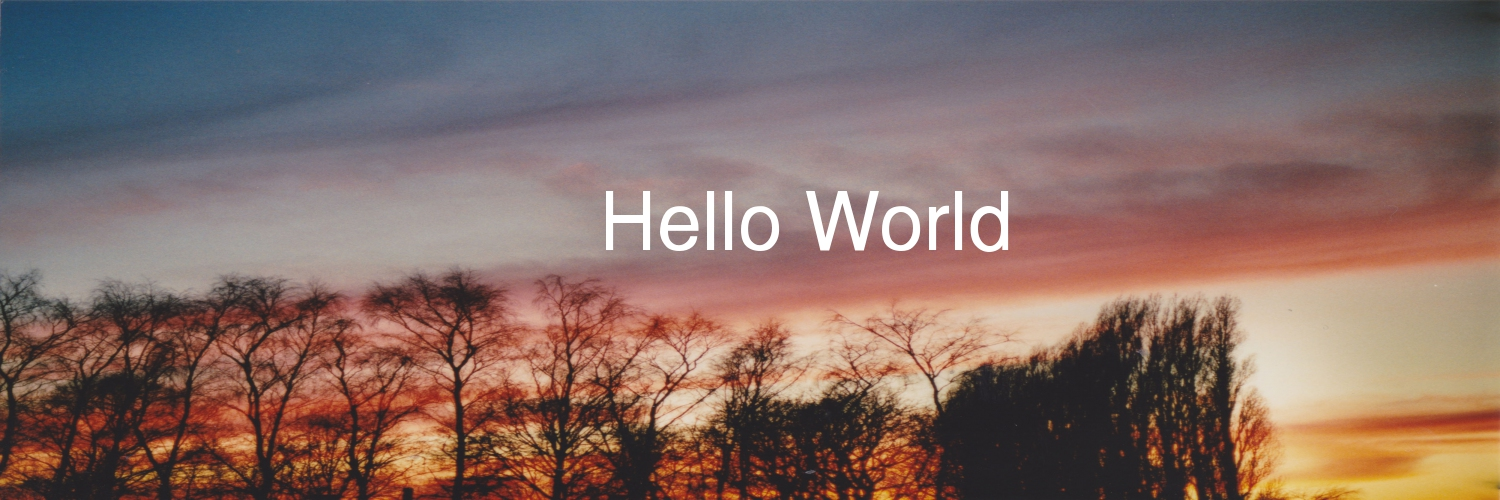
\includegraphics[width=1\textwidth]{Figuren/PHP_rendering.jpeg}
	\caption{PHP afbeelding \cite{}}
	\label{fig:PHP}
\end{figure} 
%
%https://www.thesitewizard.com/php/create-image.shtml%
%http://php.net/manual/en/book.image.php
%http://php.net/manual/en/ref.image.php
%http://jaguar.readthedocs.io/en/v1.0.0/usage/Canvas.html
%https://zinoui.com/docs/canvas

\'{E}\'{e}n van de nadelen van het gebruik van PHP is dat het object, dat ge\"{e}xporteerd wordt door de frontend, niet rechtstreeks omgezet kan worden. Ieder object in het ge\"{e}xporteerde canvas moet overlopen worden en met de juiste eigenschappen op de afbeelding geplaatst worden. Zo moet voor elk tekst object de lettergrootte, kleur, lettertype, gewicht en tekst uit de JSON representatie van het canvas gehaald worden. In het geval van een KPI moet dan ook de tekst vervangen worden. Hoewel dit perfect mogelijk is, is het niet erg efficient en zelfs wat omslachtig. Ook kan het voorkomen dat bepaalde eigenschappen niet ondersteund of anders ge\"{i}mplementeerd zijn. 

\subsection{Node.js}
Veel gemakkelijker is het gebruiken van Node.js. Hiermee kan in de backend gebruik gemaakt worden van JavaScript code. Dit betekend dat dezelfde bibliotheken, die gebruikt worden om in de frontend de afbeeldingen te editeren, gebruikt kunnen worden in de backend. Het merendeel van de eerder besproken JavaScript bibliotheken bezit ondersteuning voor Node.js. 

Omdat alle Fabric, Konva en Easel allen gebaseerd zijn op het HTML canvas element, moet ook een canvas implementatie aanwezig zijn voor Node.js. De \lstinline{npm-canvas} \textit{package} is gebaseerd op Cairo, een 2D \textit{graphics} bibliotheek geschreven in C. %https://github.com/Automattic/node-canvas 
Konva, Fabric en Easel werken in een Node omgeving hetzelfde als in een frontend omgeving. Een canvas wordt aangemaakt waaraan afbeeldingen, tekst, vormen en animaties toegevoegd kunnen worden. Zowel met Fabric als met Konva is het mogelijk om geserialiseerde data, in JSON formaat, terug om te zetten in een canvas. Bij Easel moeten alle objecten in het canvas opnieuw opgebouwd worden aangezien het met deze bibliotheek niet mogelijk is om JSON data om te zetten naar een canvas. 

Het omzetten van een JSON data naar een afbeelding gebeurt als volgt:
\textbf{Fabric.js}
\begin{lstlisting}[language=javascript]
	var fabric = require('fabric').fabric;
	var fs = require('fs');
	var data = {...};
	
	var canvas = fabric.createCanvasForNode(1500, 500);
	canvas.loadFromJSON(data, function() {
		canvas.renderAll();
	});
	
	var stream = canvas.createPNGStream();
	
	
	var out = fs.createWriteStream(__dirname + '/test-' + service + '.png');
\end{lstlisting}
\textbf{Konva.js}
\begin{lstlisting}[language=javascript]
	
	var canvas = Konva.Node.create(data, 'container');

\end{lstlisting}
\textbf{Easel.js}
\begin{lstlisting}[language=javascript]
// MISSCHIEN HIER CODE VOORBEELDJE FZO?
\end{lstlisting}

Zoals te zien in de voorbeeldcode bezit Fabric methodes specifiek voor gebruik met Node.js. De \lstinline{createCanvasForNode} methode maakt een canvas aan zonder dat hiervoor een HTML canvas element nodig is. De \lstinline{createPNGStream} methode geeft een Node Stream object terug, waarmee het canvas opgeslagen kan worden als een PNG bestand. Het Stream object kan ook de data teruggeven in een base64 formaat. Aangezien dit eenvoudigweg een tekstuele representatie van binaire data is, is dit uitermate geschikt voor dit project. Wordt een Node.js service opgezet, die als input JSON data verwacht. Dan kan de response de base64 ge\"{e}ncodeerde afbeelding bevatten. Zo wordt het mogelijk om de afbeelding bijvoorbeeld naar Facebook of Twitter te uploaden. 

Konva....

Easel....



(zie sectie \ref{vereisten})

\newpage
\section{Functioneel ontwerp}

\newpage
\section{Afbeelding compressie}

\chapter{Praktische uitwerking}
\vspace{-3cm}
\section{Frontend implementatie}
\section{Backend implementatie}


%
%\begin{table}[ht!]
%\begin{center}
%\begin{tabular}[c]{clllc}
%\hline
%Schaalwaarde & Product & Merk of soort & Staalgrootte & Temperatuur\\
%\hline
%1 & Roomkaas & Kraft Philadelphia & 1.5 cm\textsuperscript{2} & 7-13\degree~C\\
%2 & Wit van ei & Hardgekookt(5 min.) & Tipje van 1.5 cm &	20-25\degree~C\\
%3	& Frankfurterworst &	Schneiders, groot	& Sneetje van 1.5 cm	& 10-18\degree~C\\
%4	& Kaas &	Kraft mild Cheddar & 1.5 cm\textsuperscript{2} & 10-18\degree~C\\
%5	& Olijven	& McLaren's, gevuld	& 1 olijf zonder pit &	10-18\degree~C\\
%6	& Pindanoten	& Cocktail-type &	1 noot & 20-25\degree~C\\
%7	& Wortelen	& Ongekookt, vers	& Sneetje van 1.5 cm	& 20-25\degree~C\\
%8	& Amandelen	& McNair, geblancheerd &	1 noot	& 20-25\degree~C\\
%9	& Pepermuntbal	& McCormick	& 1	& 20-25\degree~C\\
%\hline
%\end{tabular}
%\caption{Voorbeeld hardheidsschaal. Naar Szczesniak (1963)} % hade moet bron nog vermelden
%\label{tabeltextureprofiling}
%\end{center}
%\end{table} 
%
%\begin{figure}[ht!]
	%\centering
		%\includegraphics[width=0.50\textwidth]{Figuren/Kwantitatievedescriptieveanalyse.pdf}
		%\caption{Voorbeeld van een kwantitatieve descriptieve analyse tussen product A en product B, twee soorten sinaasappelgelei. Naar \cite{lawless2010sensory}}
	%\label{fig:Kwantitatievedescriptieveanalyse}
%\end{figure}
